\documentclass{article}

\usepackage[utf8]{inputenc}
\usepackage[brazilian]{babel}
\usepackage{graphicx}
\usepackage{float}
\usepackage[pdftex]{hyperref}
\usepackage{epstopdf}
\usepackage{etoolbox}
\usepackage{amsmath}
\usepackage{amsfonts}
\usepackage{amssymb}
\usepackage{caption}
\usepackage{subcaption}
\usepackage{setspace}
\usepackage{tikz}
\usepackage{listings}
\usepackage{xcolor} 

\patchcmd{\thebibliography}{\section*}{\section}{}{}
\newcommand{\R}{\ensuremath{\mathbb{R}}}
\newcommand{\Prob}{\ensuremath{\mathbb{P}}}
\newcommand{\K}{\ensuremath{\mathbb{K}}}
\newcommand{\U}{\ensuremath{\mathbb{U}}}
\newcommand{\N}{\ensuremath{\mathbb{N}}}
\newcommand{\Lg}{\ensuremath{\mathbb{L}}}
\newcommand{\T}{\ensuremath{\rm Tr}}
\newcommand{\sg}{{\sigma(x_k)}}

\newcommand{\G}{\ensuremath{\mathcal{G}}}
\newcommand{\F}{\ensuremath{\mathcal{F}}}
\newcommand{\C}{\ensuremath{\mathcal{C}}}
\newcommand{\E}{\ensuremath{\mathcal{E}}}
\newcommand{\Hn}{\ensuremath{\mathcal{H}}}
%\newcommand{\Hoo}{\ensuremath{\mathcal{H}_\infty}}
\newcommand{\Hop}{\ensuremath{\mathcal{H}_{op}}}
% --------------------------------------------------
\newtheorem{theo}{Teorema}
\newtheorem{exa}{Exemplo}
\newtheorem{lemm}{Lema}
\newtheorem{coro}{Corolário}
\newtheorem{defn}{Definição}[section]

%opening
\lstset{ %
	backgroundcolor=\color{white},   % choose the background color; you must add \usepackage{color} or \usepackage{xcolor}
	basicstyle=\footnotesize,        % the size of the fonts that are used for the code
	breakatwhitespace=false,         % sets if automatic breaks should only happen at whitespace
	breaklines=true,                 % sets automatic line breaking
	captionpos=t,                    % sets the caption-position to bottom
	commentstyle=\color{green},    % comment style
	extendedchars=true,              % lets you use non-ASCII characters; for 8-bits encodings only, does not work with UTF-8
	frame=single,                    % adds a frame around the code
	keepspaces=true,                 % keeps spaces in text, useful for keeping indentation of code (possibly needs columns=flexible)
	keywordstyle=\color{cyan},       % keyword style
	language=C,                 % the language of the code
	numbers=left,                    % where to put the line-numbers; possible values are (none, left, right)
	numbersep=5pt,                   % how far the line-numbers are from the code
	numberstyle=\tiny\color{black}, % the style that is used for the line-numbers
	rulecolor=\color{gray},         % if not set, the frame-color may be changed on line-breaks within not-black text (e.g. comments (green here))
	showspaces=false,                % show spaces everywhere adding particular underscores; it overrides 'showstringspaces'
	showstringspaces=false,          % underline spaces within strings only
	showtabs=false,                  % show tabs within strings adding particular underscores
	stepnumber=2,                    % the step between two line-numbers. If it's 1, each line will be numbered
	stringstyle=\color{red},     % string literal style
	tabsize=2,                       % sets default tabsize to 2 spaces
	basicstyle=\color{black}
}

\makeatletter
\def\code{\@ifnextchar[{\@with}{\@without}}%
\def\@with[#1]#2{%
}
\def\@without#1{%
	\subsection{\protect\detokenize{#1}}%
	\lstinputlisting[language=C]{#1}%
}
\makeatother

\begin{document}

\begin{titlepage}
\begin{center}

\newcommand{\HRule}{\rule{\linewidth}{0.5mm}}
% Upper part of the page. The '~' is needed because \\
% only works if a paragraph has started.

\includegraphics[width=0.15\textwidth]{logoUnicamp}~\\[1cm]

\textsc{\LARGE Universidade Estadual de Campinas}\\[1.5cm]

\textsc{\Large Faculdade de Engenharia Mecânica}\\[0.5cm]

% Title
\HRule \\[0.4cm]
{ \huge \bfseries ES670 - Projeto de Sistemas Embarcados\\ \vspace{1cm} Relatório - Projeto Prático Parte 3\\
\Large{Requisito 3: Display LCD} \\[0.4cm] }

\HRule \\[1.5cm]

% Author and supervisor
\begin{minipage}{0.6\textwidth}
\begin{flushleft} \large
\emph{Nome:}\\
Daniel Dello Russo Oliveira\\Davi Rodrigues
\end{flushleft}
\end{minipage}
\begin{minipage}{0.2\textwidth}
\begin{flushright} \large
\emph{RA}\\ 101918\\116581
\end{flushright}
\end{minipage}

\vfill

% Bottom of the page
{\large \today}

\end{center}
\end{titlepage}


\onehalfspacing
\section{Objetivo} 
O objetivo do projeto é, de maneira incremental, implementar no target os requisitos apresentados no roteiro\cite{bb:roteiro} inicialmente desenvolvendo o modelo e depois implementando cada requisito. Estes requisitos são referentes à configuração e implementação de entradas de teclado, acionamento de LEDs, display de sete segmentos, protocolo de comunicação, display LCD, medição de velocidade de rotação, PWM, ADC e Controlador. 
	
\section{Modelagem}
% Diagramas requisitos implementados, digrama de blocos, etc
Utilizando o Rational Rhapsody Modeler e tomando como base os requisitos propostos mostrados na figura \ref{fig:requisitos}, complementamos o modelo inicial\cite{bb:modelo} (requisitos de teclado e LEDs) adicionando um bloco ao modelo referente aos displays de sete segmentos (REQ1C), conforme mostrado na figura \ref{fig:blocos}. Adicionamos também alguns blocos auxiliares relacionados ao gerenciamento de pinos GPIO, e a interrupções periódicas, que foram utilizados para nossa implementação do display de sete segmentos e do buzzer. Ao tratar o gerenciamento do display e do buzzer através de interrupções, livramos a thread principal para que essa lide com outros problemas sem precisar se preocupar com a atualização periódica dos displays.

\begin{figure}[H]
	\centering
	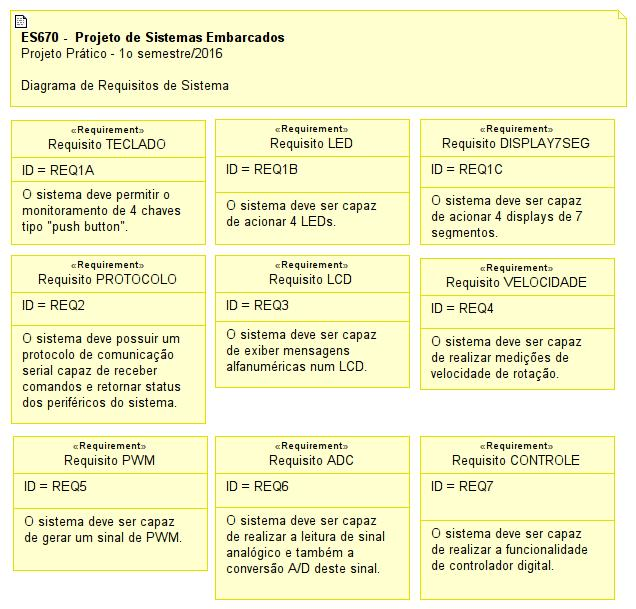
\includegraphics[width=0.9\linewidth]{requisitos}
	\caption{Diagrama de requisitos}
	\label{fig:requisitos}
\end{figure}
\begin{figure}[H]
	\centering
	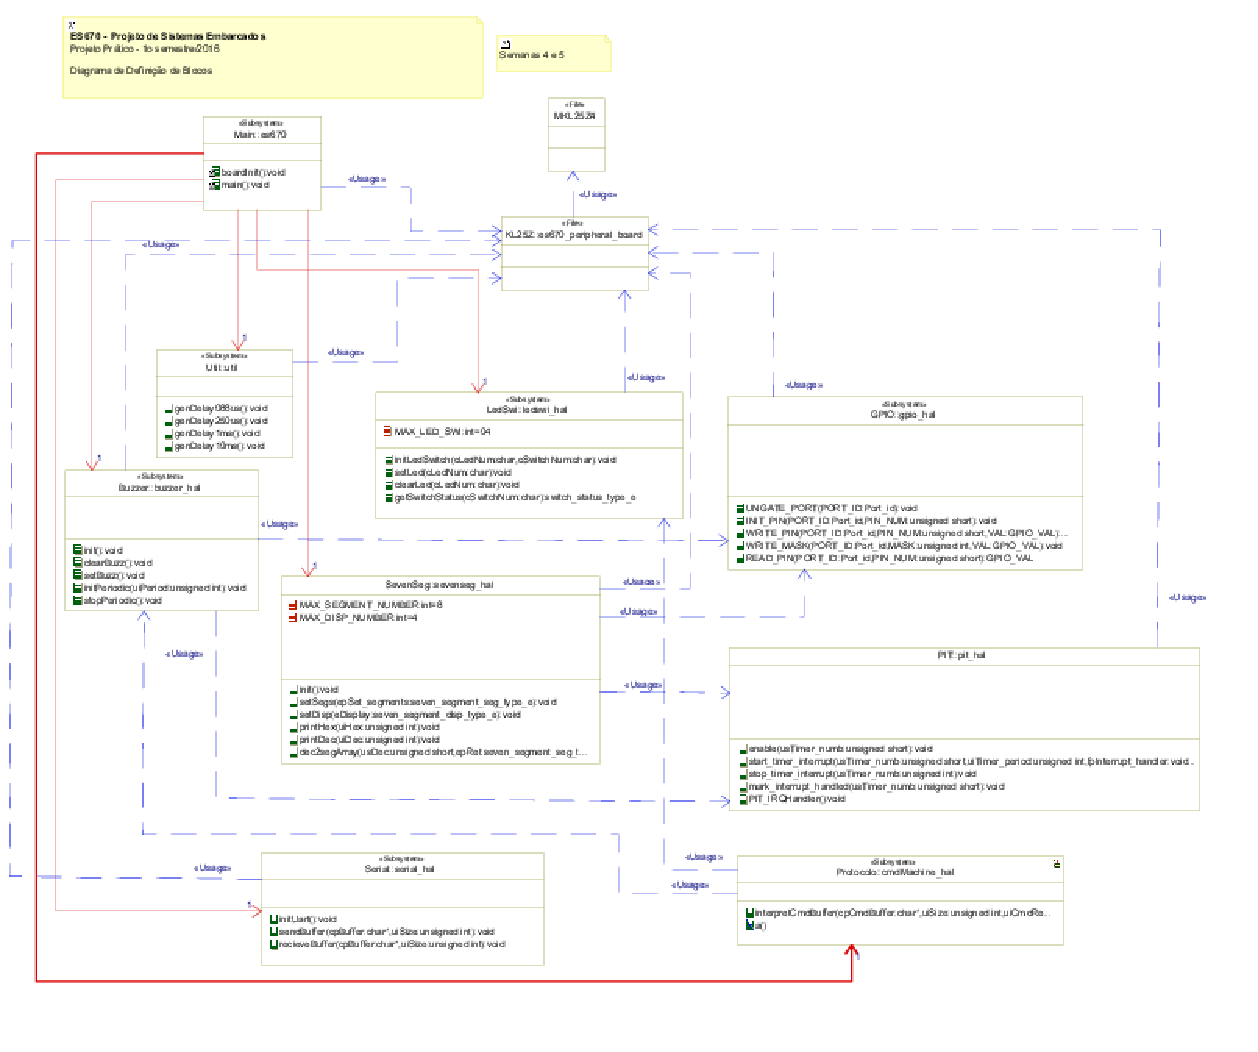
\includegraphics[width=0.9\linewidth]{blocos}
	\caption{Diagrama de definição de blocos}
	\label{fig:blocos}
\end{figure}
O bloco SevenSeg possui três operações: inicialização, definição de saída (recebendo qual dos displays será usado e qual valor deve ser exibido) e definição de saída com inteiro (recebendo apenas o valor inteiro a ser exibido no conjunto de quatro displays).

\section{Diagramas Esquemáticos}
% Diagramas esquemáticos do target utilizados

\begin{figure}[H]
	\centering
	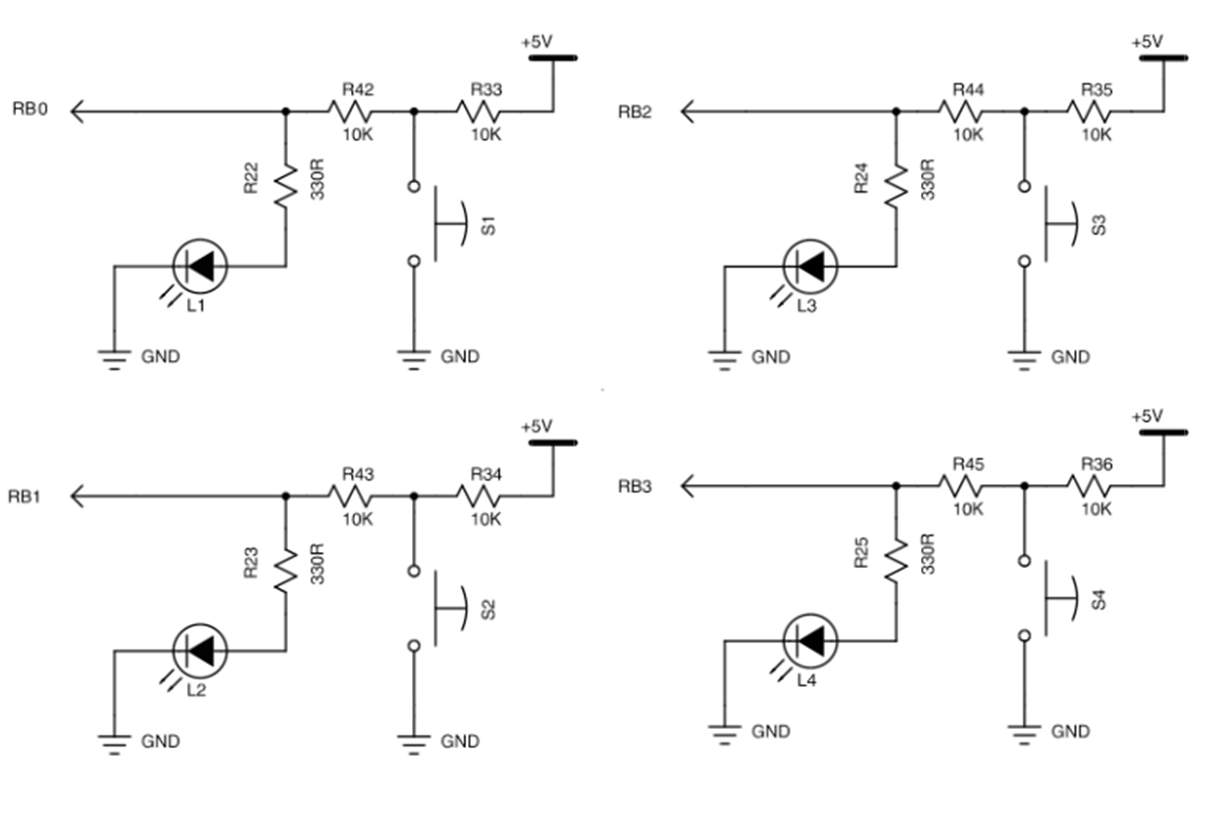
\includegraphics[width=0.7\linewidth]{esq_ledswi}
	\caption{Esquema teclado e LEDs}
	\label{fig:esq_ledswi}
\end{figure}
\begin{figure}[H]
	\centering
	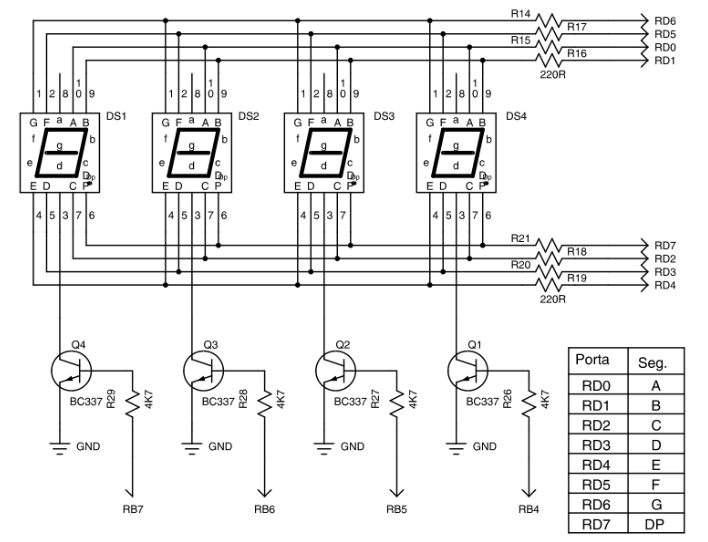
\includegraphics[width=0.9\linewidth]{esq_7seg}
	\caption{Esquema sete segmentos}
	\label{fig:esq_7seg}
\end{figure}
Como pode ser visto na figura \ref{fig:esq_7seg}, é necessário fazer um gerenciamento dos pinos PTC-0 a PTC-7 para selecionar os segmentos que serão ativados e PTC-10 a PTC-13 para selecionar quais displays estarão ativos. Para isso, é preciso alternar qual display está ativo fazendo a mudança nos segmentos para que cada display esteja mostrando um valor diferente. É importante lembrar que a frequência dessa alternância seja escolhida de modo que o olho humano não perceba que os displays estão ligando e desligando. Afim de garantir que essa alternância funcionará apropriadamente nós utilizamos o módulo PIT para gerar uma interrupção a cada 3.125 ms, conforme sugerido na aula 6 \cite{bb:aula6}. 


\section{Matriz de Rastreabilidade}
% Matriz de rastreabilidade de requisitos vs implementações
A matriz de rastreabilidade apresentada na tabela \ref*{tab:rastreabilidade} relaciona cada um dos requisitos com a sua implementação.
\begin{table}[H]
	\centering
	\caption{Matriz de Rastreabilidade}
	\label{tab:rastreabilidade}
	\small
	\begin{tabular}{|c|l|}
		\hline \bfseries{ID do Requisito} & \bfseries{Implementação}\\ 
		\hline REQ1A 	& \texttt{ledswi.c}\\ 
						& \texttt{- void ledswi\_initLedSwitch(char cLedNum, char cSwitchNum)}\\
						& \texttt{- switch\_status\_type\_e ledswi\_getSwitchStatus(char cSwitchNum)}\\
		\hline REQ1B 	& \texttt{ledswi.c}\\ 
						& \texttt{- void ledswi\_initLedSwitch(char cLedNum, char cSwitchNum)}\\
						& \texttt{- void ledswi\_setLed(char cLedNum)}\\ 
						& \texttt{- void ledswi\_clearLed(char cLedNum)}\\
		\hline REQ1C 	& \texttt{sevenSeg.c}\\ 
						& \texttt{- void sevenseg\_init(void)}\\
						& \texttt{- void sevenseg\_set(char cSSNum, sevenseg\_value\_e eValue)}\\
						& \texttt{- void sevenseg\_setWithInt (int iValue)}\\
		\hline 
	\end{tabular} 
	\normalsize
\end{table}
\section{Notas}
% Dificuldades, observações relevantes, correções, ...
Detectamos logo no início do projeto um defeito estrutural no código fornecido quando lidando com GPIO, o identificador da porta e o número do pino utilizado eram referenciados em diversos locais diferentes do código, dificultando de maneira agravante mudanças na configuração de hardware. Para resolver isso, inicialmente pensamos em utilizar o arquivo \i{fsl\_gpio\_hal.h} da biblioteca da \i{FRDM-Kl25Z}, como isso não nos foi permitido e calcular as posições na memória de cada registrador seria reimplementar a biblioteca, escolhemos por criar macros que geram o mesmo estilo de código utilizado no exemplo fornecido, utilizando o operador do pré processador de concatenação \#\#. Porém, esse operador apresenta algumas particularidades, por exemplo macros que o utilizam no seu corpo não tem seus argumentos expandidos \cite{bb:preprocessor}, para circular essa dificuldade criamos uma outras macros que funcionam como uma \i{wrappers} para essas macros, fazendo assim que seus argumentos sejam expandidos antes da chamada da concatenação. As macros que fazem a concatenação propriamente ditas não devem ser chamadas pelo usuário (sendo identificadas por um \_ no início de seus nomes).
Outra dificuldade relacionada à esse módulo é que a expansão dos argumentos das macros não parava quando chegava no identificador das portas (A,B,C,D,E), para contornar esse problema utilizamos \i{typedefs} para definir esses identificadores como parte do código.

Outro problema que enfrentamos foi com a implementação das interrupções por timer através do PIT, notavelmente pela dificuldade de encontrar uma documentação clara sobre o NVIC e pelo fato da documentação fornecida inverter a endianness em relação aos registradores de GPIO quando se refere aos registradores do PIT.

Ainda enfrentamos dificuldades com a leitura dos botões por poling, uma vez que embora implementada pelo professor e não alterada em nosso código, ela não parece funcionar apropriadamente, sendo um sintoma enfrentado por alguns de nossos colegas também.

Não conseguimos nos adaptar ao estilo de comentários sugerido pelo professor, que nos parece introduzir uma quantidade desnecessária de burocracia. Formatar todos os comentários para caber dentro daquele quadrado tomava mais tempo que a implementação do código e muita informação redundante estava sendo inserida (bastava ler a interface da função para saber seu nome e o tipo de seus argumentos). Escolhemos então substituir todos os comentários do código pelo padrão javadoc, com o qual estamos mais familiarizados e acreditamos que é capaz de documentar de maneira eficiente o código.

Também tivemos grandes dificuldades com a instalação do Rhapsody Rational Modeler no Linux (através do Wine).

\begin{thebibliography}{widestlabel}
	\bibitem{bb:roteiro}{Roteiro de Laboratório - Semanas 04 e 05 (disponibilizado para os alunos)}
	\bibitem{bb:modelo}{Projeto do Modelo Inicial do Sistema (disponibilizado para os alunos)}
	\bibitem{bb:codigo}{Código Fonte Inicial em Linguagem C (disponibilizado para os alunos)}
	\bibitem{bb:preprocessor}{The C Preprocessor (Concatenation) \url{https://gcc.gnu.org/onlinedocs/cpp/Concatenation.html#Concatenation}}
\end{thebibliography}

\section{Apêndice}
% Colocar como apêndice toda a listagem do código fonte
Listagem dos códigos fonte:
\code{../Sources/LedSwi/ledswi_hal.h}
\code{../Sources/LedSwi/ledswi_hal.c}
\code{../Sources/Mcg/mcg_hal.h}
\code{../Sources/Mcg/mcg_hal.c}
\code{../Sources/PIT/pit_hal.h}
\code{../Sources/PIT/pit_hal.c}
\code{../Sources/SevenSeg/sevenseg_hal.h}
\code{../Sources/SevenSeg/sevenseg_hal.c}
\code{../Sources/GPIO/gpio_hal.h}
\code{../Sources/Main/es670.c}
\code{../Sources/Buzzer/buzzer_hal.c}
\code{../Sources/Buzzer/buzzer_hal.h}
\code{../Sources/KL25Z/es670_peripheral_board.h}
\code{../Sources/Util/util.h}
\code{../Sources/Util/util.c}
\end{document}

